
\chapter{Giới thiệu chung}

\section{Đặt vấn đề}
Trong các doanh nghiệp, các các lập trình viên chịu trách nhiệm viết code cho dự án, còn các kỹ sư vận hàng và triển khai hạ tầng đảm nhận việc lấy mã nguồn và triển khai. Khi chỉ có một hoặc hai mã nguồn, việc triển khai chưa quá phức tạp. Tuy nhiên, thực tế một doanh nghiệp có thể có hàng chục, thậm chí hàng trăm mã nguồn. Chỉ riêng với 20 dự án trên \textbf{Git}, đã đặt ra câu hỏi: cần bao nhiêu kỹ sư vận hàng và triển khai hạ tầng để triển khai kịp tiến độ?
Quá trình phát triển dự án thường diễn ra trên ba môi trường chính:
\begin{itemize}
	\item \textbf{Development}: Môi trường để lập trình viên cập nhật các đoạn mã nguồn mới
	\item \textbf{Staging}: Môi trường kiểm thử, đảm bảo mọi thứ chạy ổn trước khi lên production và thường được các tester sử dụng.
	\item \textbf{Production}: Môi trường phục vụ người dùng cuối.
\end{itemize}



Trong môi trường \textbf{Development}, các lập trình viên cập nhật mã nguồn  hàng giờ, thậm chí hàng phút, và họ cần kiểm tra mã nguồn trên môi trường kiểm thử trước khi chuyển sang các môi trường quan trọng hơn. Nếu phải chờ các kỹ sư triển khai thủ công, điều này sẽ rất tốn thời gian và ảnh hưởng đến hiệu suất dự án.
Không chỉ lập trình viên gặp khó khăn, đội ngũ vận hàng và triển khai cũng gặp nhiều trở ngại khi triển khai thủ công: sao chép mã nguồn giữa các máy chủ có thể dẫn đến sai sót; họ phải truy cập từng máy chủ, \textbf{clone} mã nguồn, \textbf{build}, \textbf{run}, rồi kiểm tra \textbf{logs}… Ngoài ra, triển khai dự án còn bao gồm nhiều công việc khác như cài đặt hệ thống, giám sát, bảo trì và nâng cấp, làm quá trình triển khai trở nên phức tạp và tốn thời gian.

\section{Khái niệm CI/CD}

\begin{figure}[htbp]
	\centering
	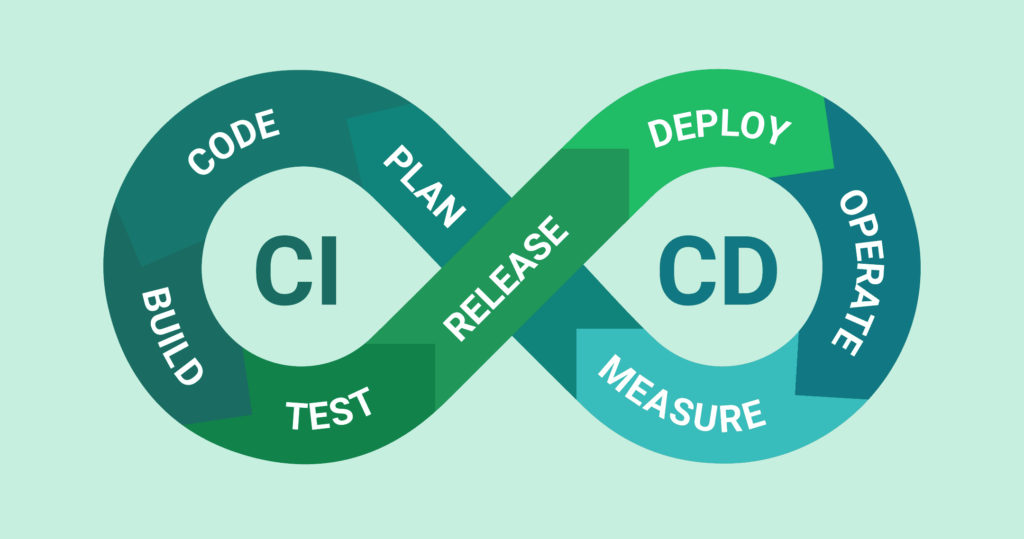
\includegraphics[width=1\linewidth]{Ảnh/defination-ci-cd.png}
	\caption{Mô Hình CI/CD}
	\label{fig:Mô Hình CI/CD}
\end{figure}


Để giải quyết các khó khăn trong phần trên, \textbf{CI/CD} ra đời.\textbf{ CI/CD} gồm hai phần chính:



\subsection*{CI (Continuous Integration)}

Bước CI bao gồm: clone mã nguồn, build dự án, và tích hợp các bước kiểm thử như:
\begin{enumerate}
	\item Kiểm tra hiệu năng 
	\item Kiểm tra chất lượng mã nguồn
	\item Kiểm tra bảo mật
	\item Và nhiều loại kiểm thử khác
\end{enumerate}
Mục tiêu là đảm bảo chất lượng mã nguồn trước khi triển khai.

\subsection*{CD (Continuous Deployment / Continuous Delivery)}
\begin{itemize}
	\item \textbf{Continuous Deployment}: triển khai hoàn toàn tự động. Lập trình viên chỉ cần commit code, chức năng mới sẽ được triển khai ngay mà không cần thao tác thủ công.
	\item \textbf{Continuous Delivery}: triển khai vẫn yêu cầu bước xác nhận thủ công. Code sau khi \textbf{build} và kiểm thử chỉ được triển khai khi có sự đồng ý từ team.
\end{itemize}



Mỗi chiến lược \textbf{CD} có ưu nhược điểm riêng:
\begin{itemize}[label=\textendash] 
	\item 	Triển khai tự động tối ưu hiệu suất và rút ngắn thời gian ra môi trường thực tế.
	\item Triển khai thủ công giúp tăng khả năng kiểm soát, giảm rủi ro lỗi khi đưa code vào môi trường quan trọng.
	Tùy theo nhu cầu doanh nghiệp, có thể kết hợp cả hai để xây dựng quy trình \textbf{CI/CD} tối ưu, vừa nhanh, vừa an toàn.
\end{itemize}


\section{Ưu điểm và hạn chế của quy trình CI/CD}

\subsection*{Ưu điểm}

	Việc triển khai quy trình \textbf{CI/CD} mang lại nhiều lợi ích rõ rệt cho đội ngũ phát triển phần mềm:

\begin{enumerate}
	\item \textbf{Giảm thiểu lỗi không đáng có:}  
	Nhờ có CI/CD, các lỗi như lỗi biên dịch hoặc lỗi phát sinh do khác biệt môi trường build được phát hiện sớm.  
	Ví dụ: cùng một source code nhưng khi bạn A build trên máy của mình và bạn B build trên máy khác có thể cho ra kết quả khác nhau.  
	Với \textbf{CI/CD}, tất cả đều được build trong môi trường thống nhất, giúp loại bỏ rủi ro này.
	
	\item \textbf{Đảm bảo tính ổn định và logic của hệ thống:}  
	Các bài kiểm thử tự động giúp bảo đảm rằng việc thêm tính năng mới không ảnh hưởng đến các chức năng hiện có.
	
	\item \textbf{Tăng hiệu quả làm việc:}  
	Kỹ sư vận hành và hạ tầng không cần tự build hay deploy ứng dụng nữa, vì mọi thao tác đã được tự động hóa.  
	Điều này giúp họ tập trung hơn vào việc phát triển và cải thiện chất lượng phần mềm.
	
	\item \textbf{Nâng cao chất lượng mã nguồn:}  
	CI/CD cho phép thiết lập các quy tắc ngay từ đầu, chẳng hạn như giới hạn kích thước của pull request hoặc số lượng thay đổi tối đa.  
	Nhờ vậy, quy trình đánh giá mã nguồn trở nên rõ ràng và chất lượng mã nguồn được cải thiện.
	
	\item \textbf{Phát triển kỹ năng viết Unit Test:}  
	Khi pipeline có chỉ số ràng buộc về \textit{code coverage}, Developer cần đảm bảo phần code mới có đủ kiểm thử để không làm giảm tỷ lệ bao phủ.  
	Điều này giúp các developer hình thành thói quen viết Unit Test và nâng cao kỹ năng kiểm thử tự động.
	
	\item \textbf{Tối ưu tốc độ phát triển sản phẩm:}  
	CI/CD cho phép theo dõi chi tiết thời gian build, test hay lint check, giúp nhóm phát triển dễ dàng phát hiện và tối ưu các khâu còn chậm.
\end{enumerate}

\subsection*{Hạn chế}

Bên cạnh những ưu điểm nổi bật, CI/CD cũng có một số hạn chế cần lưu ý:

\begin{enumerate}
	\item \textbf{Xung đột khi nhiều lập trình viên cùng làm việc:}  
	Khi có nhiều pull request cần merge vào branch, pipeline có thể bị tắc nghẽn.  
	Các thành viên phải chờ người khác merge xong, sau đó cập nhật lại code nếu có conflict và chạy test lại từ đầu, gây gián đoạn quá trình phát triển.
	
	\item \textbf{Phụ thuộc vào dịch vụ bên thứ ba:}  
	Nếu tổ chức sử dụng nền tảng CI/CD của bên ngoài như Jenkins Cloud, GitLab CI hoặc GitHub Actions,  
	khi dịch vụ gặp sự cố hoặc ngừng hoạt động, toàn bộ pipeline sẽ bị ảnh hưởng, làm gián đoạn quá trình phát triển phần mềm.
\end{enumerate}


\section{Cách thức hoạt động của quy trình CI/CD}

\begin{figure}[htbp]
	\centering
	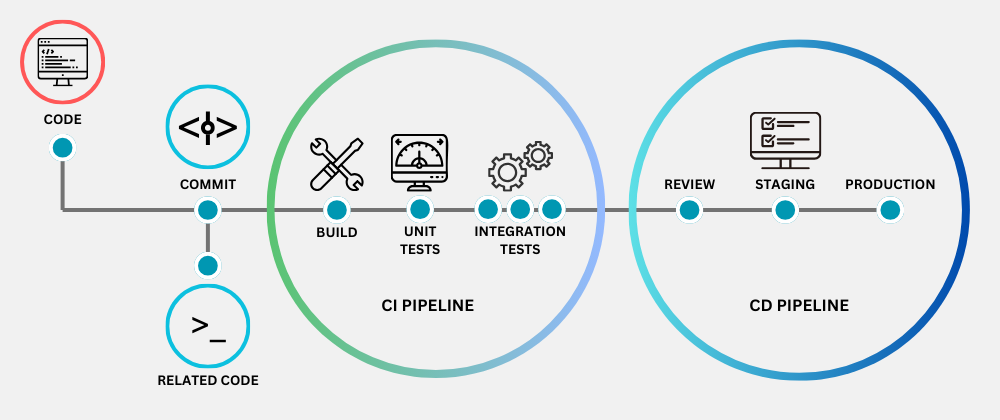
\includegraphics[width=1\linewidth]{Ảnh/ci-cd-pipeline.png}
	\caption{Quy trình CI/CD}
	\label{fig:Quy trình CI/CD}
\end{figure}


Quy trình CI/CD được vận hành thông qua sự phối hợp giữa hai thành phần chính:
\begin{enumerate}
	\item \textbf{Git Repository} – nơi lưu trữ mã nguồn và quản lý toàn bộ thay đổi trong dự án.
	\item \textbf{CI/CD Tool} – công cụ đảm nhiệm việc tự động hóa các giai đoạn như build, test, deploy và theo dõi kết quả.
\end{enumerate}

Cụ thể, khi một Developer thực hiện thay đổi trong Git repository (ví dụ: tạo \textit{pull request} hoặc \textit{commit} mới), Git sẽ gửi thông báo đến CI/CD tool rằng có cập nhật mới được tạo. Ngay sau đó, CI/CD tool tự động kích hoạt pipeline và chạy tuần tự các bước đã được cấu hình sẵn, thường bao gồm:

\begin{itemize}
	\item \textbf{Biên dịch mã nguồn (Build):} Toàn bộ mã nguồn được biên dịch để kiểm tra tính hợp lệ, đảm bảo không có lỗi cú pháp hoặc lỗi phụ thuộc thư viện.
	\item \textbf{Kiểm thử tự động (Testing):} Hệ thống thực hiện các bài kiểm thử đơn vị (unit test), kiểm thử tích hợp (integration test), hoặc kiểm thử giao diện (UI test) để đảm bảo logic chương trình hoạt động đúng.
	\item \textbf{Phân tích chất lượng mã (Static Code Analysis):} Mã nguồn được kiểm tra bằng các công cụ như SonarQube, ESLint hoặc Checkstyle để phát hiện lỗi tiềm ẩn, vi phạm quy tắc code, hoặc các rủi ro bảo mật.
	\item \textbf{Kiểm tra quy tắc (Code Policy Check):} Pipeline xác minh các quy định nội bộ như kích thước \textit{pull request}, quy ước đặt tên, hay tiêu chuẩn lập trình.
\end{itemize}

\subsection*{Giai đoạn sau kiểm thử (Post-testing stage)}

Khi toàn bộ các bài kiểm thử và kiểm tra chất lượng mã đều đạt yêu cầu, CI/CD tool sẽ tự động chuyển sang các bước xử lý tiếp theo:

\begin{enumerate}
	\item \textbf{Đóng gói và build artifact:}  
	Mã nguồn sau khi được xác nhận hợp lệ sẽ được đóng gói thành một \textit{artifact} (ví dụ: file \texttt{.jar}, \texttt{.war}, \texttt{.zip} hoặc Docker image).  
	Artifact này được lưu trữ trong kho lưu trữ riêng (như Artifactory, Nexus hoặc Docker Registry) để phục vụ cho việc triển khai ở các môi trường tiếp theo.
	
	\item \textbf{Triển khai tự động (Deploy):}  
	Hệ thống tự động triển khai artifact vừa build lên môi trường \textit{staging} hoặc \textit{production} tùy theo cấu hình.  
	Việc deploy có thể được thực hiện thông qua các công cụ như Jenkins, GitLab CI/CD, ArgoCD hoặc Kubernetes.  
	Ở giai đoạn này, pipeline có thể tích hợp thêm các bài kiểm thử sau triển khai (post-deployment tests) nhằm xác nhận ứng dụng hoạt động đúng trên môi trường thực tế.

	
	\item \textbf{Khả năng rollback:}  
	Trong trường hợp phiên bản mới gây lỗi hoặc ảnh hưởng đến hệ thống, pipeline hỗ trợ cơ chế \textbf{rollback} để quay lại phiên bản ổn định trước đó.  
	Rollback có thể được thực hiện thủ công hoặc tự động (auto-rollback) nếu hệ thống phát hiện các chỉ số bất thường như downtime, lỗi 5xx, hoặc giảm hiệu năng.
\end{enumerate}

\subsection*{Tổng kết}

Khi toàn bộ quá trình hoàn tất, CI/CD tool phản hồi kết quả ngược lại cho Git repository, thể hiện trạng thái của \textit{pull request} hoặc \textit{commit} là thành công hoặc thất bại.  
Dựa vào đó, tester có thể dễ dàng đánh giá sơ bộ chất lượng code trước khi thực hiện đánh giá chi tiết.

Tuy nhiên, quy trình CI/CD chỉ có thể tự động hóa và kiểm soát được một phần logic kỹ thuật.  
Việc đánh code thủ công từ lập trình viên hoặc tester vẫn là bước cần thiết nhằm đảm bảo mã nguồn đáp ứng tiêu chuẩn của nhóm và xử lý được những trường hợp logic phức tạp mà hệ thống tự động chưa thể bao quát hết.

